\documentclass[a4paper,11pt]{report}

\usepackage{amsmath,amssymb}
\usepackage{fullpage}
\usepackage{graphicx}
\usepackage[cache=false]{minted}

\usepackage{bussproofs}
\usepackage{mathpartir}
\usepackage{prooftrees}
\usepackage{color}

\usepackage{tikz}
\usetikzlibrary{automata,positioning}

\newcommand*\circled[1]{\tikz[baseline=(char.base)]{
            \node[shape=circle,draw,inner sep=2pt] (char) {#1};}}

\makeatletter
\pgfmathdeclarefunction{alpha}{1}{%
  \pgfmathint@{#1}%
  \edef\pgfmathresult{\pgffor@alpha{\pgfmathresult}}%
}

\newcommand*{\until}{U}
\newcommand*{\disj}{\ ,\ }
\newcommand*{\A}{\square}  % Always
\newcommand*{\D}{\diamondsuit} % eventually

\newcommand*{\Pq}{(\top,\bot)}
\newcommand*{\pQ}{(\bot,\top)}
\newcommand*{\PQ}{(\top,\top)}
\newcommand*{\pq}{(\bot,\bot)}

\usemintedstyle{tango}

\newminted[promelacode]{C}{
  frame=single,
  framesep=6pt,
  breaklines=true,
  fontsize=\scriptsize
}

\newmintinline[promelainline]{C}{breaklines=true,fontsize=\small}

\newmintedfile{c}{frame=single, framesep=6pt, breaklines=true,fontsize=\scriptsize}
\newcommand{\ex}[3]{\cfile[firstline=#1,lastline=#2]{ex#3.pml}}

% tikz
\usepackage{tikz}
\usetikzlibrary{snakes}

\author{Sylvain Julmy}
\date{\today}

\setlength{\parindent}{0pt}
\setlength{\parskip}{2.5pt}

\begin{document}

\begin{center}
\Large{
    Verification of Cyber-Physical System\\
    Fall 2017
  }
  
  \noindent\makebox[\linewidth]{\rule{\linewidth}{0.4pt}}
  Exercice Sheet 4

  \vspace*{1.4cm}

  Author : Sylvain Julmy
  \noindent\makebox[\linewidth]{\rule{\linewidth}{0.4pt}}

  \begin{flushleft}
    Professor : Ultes-Nitsche Ulrich
    
    Assistant : Prisca Dotti
  \end{flushleft}

  \noindent\makebox[\linewidth]{\rule{\textwidth}{1pt}}
\end{center}

\section*{Exercice 1}

Using the \textit{spin} command line interface, we can automatically create a
never claim from the \textit{LTL} formula $\diamondsuit \square q$. Because it
is a never claim and we have to check that $q$ satisfies the system behavior, we
have to create the never claim with $\neg(\diamondsuit \square q)$ :

\verb|spin -f '!(<>[]q)'|

which give us the following never claim :

\begin{promelacode}
never  {    /* !(<>[]q) */
T0_init:
  do
  :: (! ((q))) -> goto accept_S9
  :: (1) -> goto T0_init
  od;
accept_S9:
  do
  :: (1) -> goto T0_init
  od;
}
\end{promelacode}

\newpage
\section*{Exercice 2}

\subsection*{(1)}

Algorithmic sugar :

\begin{center}
  \begin{forest}
    [\fbox{$a \until b$}
    [$b \vee (a \wedge X(a \until  b))$
    [\fbox{$b$}]
    [$a \wedge X(a \until b)$
    [\fbox{$a \disj  X(a \until b)$}
    [\fbox{$a \until b$} [$\cdots$]]
    ]
    ]
    ]
    ]
  \end{forest}
\end{center}

Automaton construction :

\begin{center}
  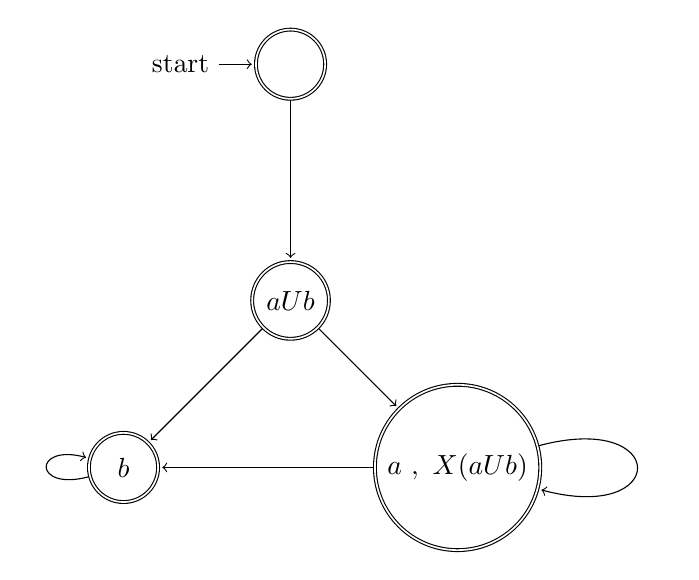
\begin{tikzpicture}[shorten >=1pt,node distance=3cm,on grid,auto]
    \node[state,accepting,initial] (init) {};
    \node[state,accepting] (a) [below = of init] {$a \until b$};
    \node[state,accepting] (b) [below left = of a] {$b$};
    \node[state,accepting] (c) [below right = of a] {$a \disj X(a \until b)$};
    \path[->]
    (init) edge node {} (a)
    (a) edge node {} (b)
        edge node {} (c)
    (b) edge [loop left] node {} ()
    (c) edge node {} (b)
        edge [loop right] node {} ();
\end{tikzpicture}
\end{center}

\newpage
\subsection*{(2)}

First, we transform

\[
  \square \diamondsuit a
\]

into

\begin{align*}
  \square \diamondsuit a &\equiv \neg \diamondsuit \neg (\diamondsuit a) \\
                         &\equiv \neg (\top \until (\neg (\diamondsuit a))) \\
                         &\equiv \neg (\top \until(\neg(\top \until a)))
\end{align*}

Algorithmic sugar (note : we simplify formulae like $\top \wedge a \equiv a$ and
$\bot \vee a \equiv a$) :

\begin{center}
  \begin{forest}
    [$ \neg (\top \until(\neg(\top \until a)))$
    [$ \neg (\neg \top \until a) \wedge (\neg \top \vee \neg X(\top \until (\neg(\top \until a))))$
    [$ \neg (\neg \top \until a) \disj (\neg \top \vee \neg X(\top \until (\neg(\top \until a))))$
    [$ \top \until a \disj \bot \vee \neg X(\top \until (\neg(\top \until a)))$
    [$ a \wedge (\top \wedge X(\top \until a)) \disj \bot \vee \neg X(\top \until (\neg(\top \until a)))$
    [$ a \disj X(\top \until a) \disj \neg X(\top \until (\neg(\top \until a)))$
    [\fbox{$ a \disj X(\top \until a) \disj X(\neg (\top \until (\neg(\top
      \until a))))$}
    [$ \top \until a \disj \neg (\top \until (\neg (\top \until a)))$
    [$ \cdots $
    ]    ]    ]    ]    ]    ]    ]    ]    ]
  \end{forest}
\end{center}


Automaton construction :

\begin{center}
  \begin{tikzpicture}[shorten >=1pt,node distance=4cm,on grid,auto]
    \node[state,initial] (init) {};
    \node[state,accepting] (a) [below = of init] {$a \disj X(\top \until a) \disj X(\neg (\top \until (\neg(\top
      \until a))))$};
    \path[->]
    (init) edge node {} (a)
    (a) edge [loop right] node {} ();
  \end{tikzpicture}
\end{center}

\section*{Exercice 3}

We denote $(\phi,\lambda)$ a moment in the timeline where $\phi$
represent $p$ and $\lambda$ represent $q$ (for example, $s_i = (\top,\bot)$
means that $p$ is true and $q$ is false at moment $i$), where $S = (s_0,s_1,\cdots,s_n,\cdots)$

\subsection*{(1)}

$\A p \vee q \not\leftrightarrow \A (p \vee q)$, because of the following
timeline :
\[
  (\Pq,\pQ,\Pq,\cdots,\Pq,\pQ,\Pq,\pQ,\cdots)
\]

$\A p \vee q$ is false at $s_0$ and $\A (p \vee q)$ is always true.

\subsection*{(2)}

$\D p \vee \D q \leftrightarrow \D (p \vee q)$ because it is just the
distributivity law of $\D$ : $\D (p \vee q) \equiv \D p \vee \D q$.

\subsection*{(3)}

$\D (p \until q) \leftrightarrow \D q$, because we don't care about $p$, if $\D
(p \until q)$ holds at a certain moment, it means that $q$ will holds at a
certain moment, which is $\D q$.

\end{document}
